% FIGURES NEEDED: none (all diagrams are TikZ)
% 11 frames total, 0 external figures
% Sources for every number: ../../notes/experiment-design-sources.md
\documentclass[11pt,aspectratio=43]{beamer}

\usepackage{amsmath,amssymb}
\usepackage{booktabs}
\usepackage{colortbl}
\usepackage{graphicx}
\usepackage{xcolor}
\usepackage{tikz}
\usepackage{hyperref}
\hypersetup{colorlinks=true,urlcolor=accent,linkcolor=accent}
\usetikzlibrary{arrows.meta,positioning,shapes.geometric,calc,decorations.pathreplacing,fit,backgrounds,patterns}

\definecolor{accent}{HTML}{2E75B6}
\definecolor{red2}{HTML}{C0392B}
\definecolor{green2}{HTML}{27AE60}
\definecolor{orange2}{HTML}{E67E22}
\definecolor{gray2}{HTML}{7F8C8D}
\definecolor{purple2}{HTML}{8E44AD}
% where things run: CPU is warm, GPU is cool, memory is neutral
\definecolor{cpuc}{HTML}{F6E9C6}
\definecolor{cpud}{HTML}{9A7420}
\definecolor{gpuc}{HTML}{D6E2EE}
\definecolor{gpud}{HTML}{3F6286}
\definecolor{memc}{HTML}{E4E4E4}

\setbeameroption{hide notes}
\setbeamertemplate{navigation symbols}{}
\setbeamersize{text margin left=0.9cm,text margin right=0.9cm}

\setbeamercolor{normal text}{fg=black,bg=white}
\setbeamercolor{frametitle}{fg=black,bg=white}
\setbeamercolor{title}{fg=black}
\setbeamercolor{structure}{fg=black}
\setbeamercolor{alerted text}{fg=accent}
\setbeamercolor{block title}{fg=black,bg=black!10}
\setbeamercolor{block body}{fg=black,bg=black!3}
\setbeamercolor{itemize item}{fg=black}
\setbeamercolor{itemize subitem}{fg=black}

\setbeamerfont{title}{size=\normalsize,series=\bfseries}
\setbeamerfont{frametitle}{size=\normalsize,series=\bfseries}
\setbeamerfont{block title}{size=\small,series=\bfseries}
\setbeamerfont{block body}{size=\small}

\setbeamertemplate{footline}{%
  \leavevmode%
  \hbox{%
    \begin{beamercolorbox}[wd=\paperwidth,ht=2.5ex,dp=1.0ex,rightskip=0.9cm]{author in head/foot}%
      \hfill\insertframenumber
    \end{beamercolorbox}%
  }%
}

\title{Latency-Bound Inference Experiments}
\author{Pulak Mehrotra}
\date{\today}

\newcommand{\question}[3]{%
  \begin{minipage}[t]{0.1\linewidth}
    {\fontsize{22}{24}\selectfont\color{accent}\bfseries #1}
  \end{minipage}%
  \begin{minipage}[t]{0.88\linewidth}
    \vspace{0.05cm}
    {\bfseries #2}\\[0.1em]
    {\small\color{gray2}#3}
  \end{minipage}}

% numbered timestamp marker, for use in running text
\newcommand{\ts}[1]{\tikz[baseline=(c.base)]\node[circle,fill=black,text=white,font=\tiny\bfseries,inner sep=0pt,minimum size=3.2mm](c){#1};}
% colour key: white box with a coloured border
\newcommand{\key}[2]{\tikz[baseline=-0.6ex]\draw[#1, line width=1.1pt, fill=white, rounded corners=1pt] (0,-0.12) rectangle (0.42,0.12);~#2}
\newcommand{\inrow}{%
  {\small\bfseries In}\par\vspace{-0.15cm}
  \begin{columns}[T,onlytextwidth]
  \column{0.31\textwidth}\begin{block}{Trace}\small synthetic, a new image every request\end{block}
  \column{0.31\textwidth}\begin{block}{Timing}\small every 1.5~s, or $k$~steps before a chunk ends\end{block}
  \column{0.31\textwidth}\begin{block}{Setup}\small the baseline, or one change from it\end{block}
  \end{columns}
  \vspace{0.15cm}
  {\centering\small $\downarrow$\quad\textbf{one run}: a few hundred requests, repeated\quad$\downarrow$\par}
  \vspace{0.1cm}}
\newcommand{\late}{\textcolor{red2}{\textbf{late}}}
\newcommand{\tight}{\textcolor{orange2}{\textbf{tight}}}
\newcommand{\fits}{\textcolor{green2!70!black}{\textbf{fits}}}

% shared TikZ styles
\tikzset{
  % what a box is: white box, coloured border
  wb/.style={draw, fill=white, rounded corners=2pt, line width=1.1pt, align=center, inner sep=3pt},
  pstep/.style={wb, draw=black!55},
  stk/.style={wb, draw=purple2},
  mdl/.style={wb, draw=accent},
  nmw/.style={wb, draw=orange2},
  simw/.style={wb, draw=green2!70!black},
  due/.style={wb, draw=red2, fill=red2!6},
  arr/.style={-{Stealth[length=5pt]}, line width=0.8pt},
  thin/.style={-{Stealth[length=4pt]}, line width=0.5pt, black!60},
  tsn/.style={circle, fill=black, text=white, font=\tiny\bfseries, inner sep=0pt, minimum size=3.4mm},
  tsw/.style={font=\scriptsize, text=black!80},
  lbl/.style={font=\scriptsize, text=black!70},
}

\begin{document}

% ==================================================================
\begin{frame}[plain]
  \titlepage
\end{frame}

% ==================================================================
\begin{frame}{One request, step by step.}

\vspace{0.35cm}
\begin{center}
\resizebox{\linewidth}{!}{%
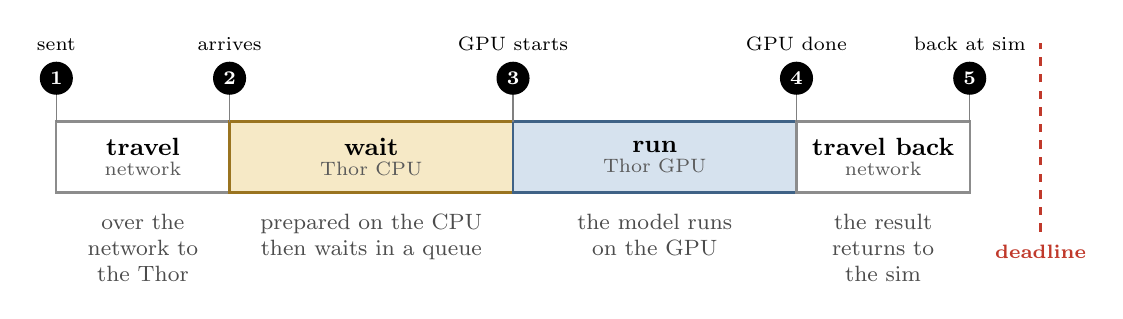
\begin{tikzpicture}[every node/.style={font=\scriptsize}]
  % the four parts of one request, coloured by where they happen
  \foreach \a/\b/\fc/\dc/\name/\where in {
      0/2.2/white/black!45/travel/network,
      2.2/5.8/cpuc/cpud/wait/Thor CPU,
      5.8/9.4/gpuc/gpud/run/Thor GPU,
      9.4/11.6/white/black!45/travel back/network} {
    \draw[fill=\fc, draw=\dc, line width=0.8pt] (\a,1.0) rectangle (\b,1.9);
    \node[align=center] at ({(\a+\b)/2},1.45) {{\small\bfseries \name}\\[-1pt]{\color{black!65}\where}};
  }
  % what happens in each part
  \foreach \a/\b/\txt in {
      0/2.2/over the network to the Thor,
      2.2/5.8/prepared on the CPU then waits in a queue,
      5.8/9.4/the model runs on the GPU,
      9.4/11.6/the result returns to the sim} {
    \node[anchor=north, align=center, text width={(\b-\a-0.2)*1cm}, text=black!70, font=\footnotesize] at ({(\a+\b)/2},0.85) {\txt};
  }
  % the five moments we time
  \foreach \x/\n/\w in {0/1/sent, 2.2/2/arrives, 5.8/3/GPU starts, 9.4/4/GPU done, 11.6/5/back at sim} {
    \draw[black!50] (\x,1.9) -- (\x,2.25);
    \node[tsn, minimum size=4.2mm, font=\scriptsize\bfseries] at (\x,2.45) {\n};
    \node[anchor=south, font=\scriptsize] at (\x,2.68) {\w};
  }
  % deadline
  \draw[red2, dashed, line width=0.9pt] (12.5,0.5) -- (12.5,2.9);
  \node[red2, font=\scriptsize\bfseries, anchor=north] at (12.5,0.45) {deadline};
\end{tikzpicture}}
\end{center}

\vspace{0.3cm}
\begin{center}
\footnotesize
\renewcommand{\arraystretch}{1.3}
\begin{tabular}{l|l|l|l}
\toprule
 & \textbf{the sim sends} & \textbf{it gets back} & \textbf{budget} \\
\midrule
Space, Gemma 3 4B & a 4K image & keep or drop & 1.5 s \\
Robot, $\pi_{0.5}$ & two camera images & 10 arm actions & 100 to 250 ms \\
\bottomrule
\end{tabular}
\end{center}

\vspace{0.2cm}
\small
A request is late when \ts{5} comes after the deadline.

\end{frame}

% ==================================================================
\begin{frame}{Where each step runs.}

\vspace{-0.1cm}
\begin{center}
\resizebox{!}{0.72\textheight}{%
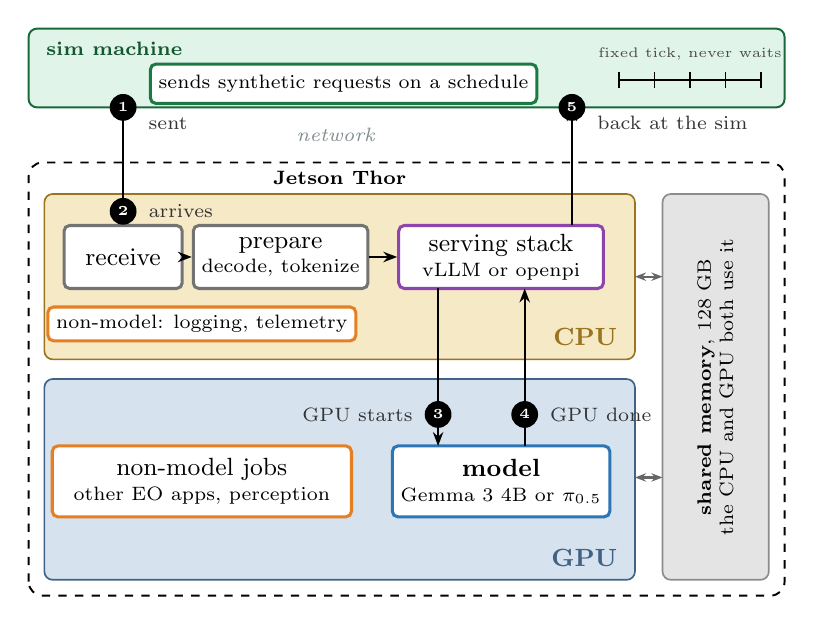
\begin{tikzpicture}[every node/.style={font=\small}]
  % ---- sim machine ----
  \draw[fill=green2!14, draw=green2!60!black, line width=0.7pt, rounded corners=3pt] (0,6.2) rectangle (9.6,7.2);
  \node[anchor=north west, font=\scriptsize\bfseries, text=green2!50!black] at (0.1,7.15) {sim machine};
  \node[simw, font=\scriptsize, minimum width=4.2cm, minimum height=0.5cm] at (4.0,6.5) {sends synthetic requests on a schedule};
  \coordinate (k0) at (7.5,6.55);
  \coordinate (k1) at (9.3,6.55);
  \draw[line width=0.6pt] (k0) -- (k1);
  \foreach \i in {0,...,4} { \draw[line width=0.6pt] ($(k0)!\i/4!(k1)$) ++(0,-0.1) -- ++(0,0.2); }
  \node[lbl, font=\tiny, anchor=south] at ($(k0)!0.5!(k1)+(0,0.13)$) {fixed tick, never waits};

  \node[font=\scriptsize\itshape, text=gray2] at (3.9,5.85) {network};

  % ---- Thor: CPU on top, GPU below, memory at the side touching both ----
  \draw[dashed, line width=0.7pt, rounded corners=5pt] (0,0) rectangle (9.6,5.5);
  \node[font=\scriptsize\bfseries] at (3.95,5.3) {Jetson Thor};

  \draw[fill=cpuc, draw=cpud, line width=0.6pt, rounded corners=3pt] (0.2,3.0) rectangle (7.7,5.1);
  \node[anchor=south east, font=\small\bfseries, text=cpud] at (7.6,3.05) {CPU};
  \draw[fill=gpuc, draw=gpud, line width=0.6pt, rounded corners=3pt] (0.2,0.2) rectangle (7.7,2.75);
  \node[anchor=south east, font=\small\bfseries, text=gpud] at (7.6,0.25) {GPU};
  \draw[fill=memc, draw=black!45, line width=0.6pt, rounded corners=3pt] (8.05,0.2) rectangle (9.4,5.1);
  \node[rotate=90, align=center, font=\scriptsize] at (8.72,2.65) {\textbf{shared memory}, 128 GB\\the CPU and GPU both use it};
  \draw[{Stealth[length=4pt]}-{Stealth[length=4pt]}, line width=0.8pt, black!60] (7.7,4.05) -- (8.05,4.05);
  \draw[{Stealth[length=4pt]}-{Stealth[length=4pt]}, line width=0.8pt, black!60] (7.7,1.5) -- (8.05,1.5);

  \node[pstep, minimum width=1.5cm, minimum height=0.8cm] (recv) at (1.2,4.3) {receive};
  \node[pstep, minimum width=2.0cm, minimum height=0.8cm] (prep) at (3.2,4.3) {prepare\\[-2pt]{\scriptsize decode, tokenize}};
  \node[stk, minimum width=2.6cm, minimum height=0.8cm] (stk) at (6.0,4.3) {serving stack\\[-2pt]{\scriptsize vLLM or openpi}};
  \node[nmw, minimum width=3.8cm, minimum height=0.42cm, font=\scriptsize] at (2.2,3.45) {non-model: logging, telemetry};

  \node[nmw, minimum width=3.8cm, minimum height=0.9cm] at (2.2,1.45) {non-model jobs\\[-2pt]{\scriptsize other EO apps, perception}};
  \node[mdl, minimum width=2.6cm, minimum height=0.9cm] (M) at (6.0,1.45) {\textbf{model}\\[-2pt]{\scriptsize Gemma 3 4B or $\pi_{0.5}$}};

  % ---- the request's path ----
  \draw[arr] (1.2,6.2) -- (recv.north);
  \draw[arr] (recv) -- (prep);
  \draw[arr] (prep) -- (stk);
  \draw[arr] (5.2,3.9) -- (5.2,1.9);
  \draw[arr] (6.3,1.9) -- (6.3,3.9);
  \draw[arr] (6.9,4.7) -- (6.9,6.2);

  \node[tsn] at (1.2,6.2) {1};   \node[tsw, anchor=west] at (1.4,6.0) {sent};
  \node[tsn] at (1.2,4.88) {2};  \node[tsw, anchor=west] at (1.4,4.88) {arrives};
  \node[tsn] at (5.2,2.3) {3};   \node[tsw, anchor=east] at (5.0,2.3) {GPU starts};
  \node[tsn] at (6.3,2.3) {4};   \node[tsw, anchor=west] at (6.5,2.3) {GPU done};
  \node[tsn] at (6.9,6.2) {5};   \node[tsw, anchor=west] at (7.1,6.0) {back at the sim};
\end{tikzpicture}}
\end{center}

\vspace{-0.1cm}
\small
The CPU and GPU are separate processors, but they share one memory.

\end{frame}

% ==================================================================
\begin{frame}{When each step runs.}

\vspace{0.1cm}
\begin{center}
\resizebox{\linewidth}{!}{%
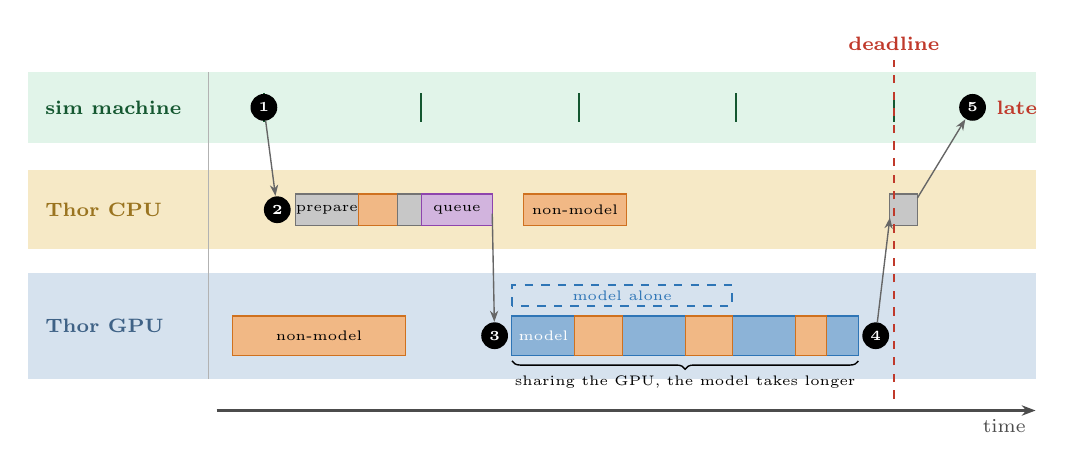
\begin{tikzpicture}[every node/.style={font=\scriptsize}]
  % lanes
  \fill[green2!14] (0,3.85) rectangle (12.8,4.75);
  \fill[cpuc] (0,2.5) rectangle (12.8,3.5);
  \fill[gpuc] (0,0.85) rectangle (12.8,2.2);
  \node[anchor=west, font=\scriptsize\bfseries, text=green2!50!black] at (0.1,4.3) {sim machine};
  \node[anchor=west, font=\scriptsize\bfseries, text=cpud] at (0.1,3.0) {Thor CPU};
  \node[anchor=west, font=\scriptsize\bfseries, text=gpud] at (0.1,1.53) {Thor GPU};
  \draw[black!30] (2.3,0.85) -- (2.3,4.75);

  % the sim keeps ticking
  \foreach \x in {3,5,7,9,11} { \draw[line width=0.7pt, green2!50!black] (\x,4.12) -- (\x,4.48); }

  % CPU: request steps share the CPU with other jobs
  \draw[fill=black!22, draw=black!55] (3.4,2.8) rectangle (4.2,3.2);   \node[font=\tiny] at (3.8,3.0) {prepare};
  \draw[fill=orange2!55, draw=orange2!90!black] (4.2,2.8) rectangle (4.7,3.2);
  \draw[fill=black!22, draw=black!55] (4.7,2.8) rectangle (5.0,3.2);
  \draw[fill=purple2!40, draw=purple2] (5.0,2.8) rectangle (5.9,3.2); \node[font=\tiny] at (5.45,3.0) {queue};
  \draw[fill=orange2!55, draw=orange2!90!black] (6.3,2.8) rectangle (7.6,3.2); \node[font=\tiny] at (6.95,3.0) {non-model};
  \draw[fill=black!22, draw=black!55] (10.95,2.8) rectangle (11.3,3.2);

  % GPU: model and non-model take turns
  \draw[fill=orange2!55, draw=orange2!90!black] (2.6,1.15) rectangle (4.8,1.65); \node[font=\tiny] at (3.7,1.4) {non-model};
  \foreach \a/\b in {6.15/6.95, 7.55/8.35, 8.95/9.75, 10.15/10.55} {
    \draw[fill=accent!55, draw=accent] (\a,1.15) rectangle (\b,1.65);
  }
  \foreach \a/\b in {6.95/7.55, 8.35/8.95, 9.75/10.15} {
    \draw[fill=orange2!55, draw=orange2!90!black] (\a,1.15) rectangle (\b,1.65);
  }
  \node[font=\tiny, text=white] at (6.55,1.4) {model};
  \draw[accent, dashed, line width=0.7pt] (6.15,1.78) rectangle (8.95,2.04);
  \node[font=\tiny, text=accent] at (7.55,1.91) {model alone};
  \draw[decorate, decoration={brace, amplitude=3pt, mirror}, line width=0.5pt] (6.15,1.08) -- (10.55,1.08)
    node[midway, below=2pt, font=\tiny] {sharing the GPU, the model takes longer};

  % timestamps
  \node[tsn] (t1) at (3.0,4.3) {1};
  \node[tsn] (t2) at (3.17,3.0) {2};
  \node[tsn] (t3) at (5.93,1.4) {3};
  \node[tsn] (t4) at (10.77,1.4) {4};
  \node[tsn] (t5) at (12.0,4.3) {5};
  \draw[thin] (t1) -- (t2);
  \draw[thin] (5.9,2.95) -- (t3);
  \draw[thin] (t4) -- (10.95,2.9);
  \draw[thin] (11.3,3.15) -- (t5);

  % deadline
  \draw[red2, dashed, line width=0.9pt] (11.0,0.6) -- (11.0,4.9);
  \node[red2, font=\scriptsize\bfseries, anchor=south] at (11.0,4.9) {deadline};
  \node[red2, font=\scriptsize\bfseries, anchor=west] at (12.18,4.3) {late};

  % time axis
  \draw[arr, black!70] (2.4,0.45) -- (12.8,0.45);
  \node[lbl, anchor=east] at (12.8,0.25) {time};
\end{tikzpicture}}
\end{center}

\vspace{0.1cm}
\small
\begin{itemize}
  \setlength{\itemsep}{0.4em}
  \item Model and non-model jobs take turns on the same CPU and GPU.
  \item Alone, the model ends at the dashed box. Sharing makes \ts{5} late.
\end{itemize}

\end{frame}

% ==================================================================
\begin{frame}{Space: one image every 1.5 seconds.}

\vspace{0.2cm}
\begin{center}
\resizebox{0.9\linewidth}{!}{%
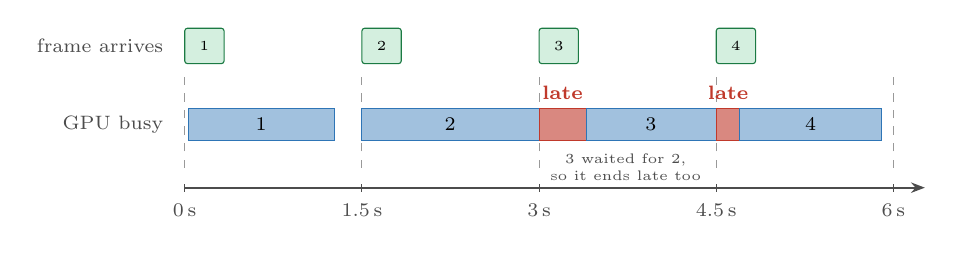
\begin{tikzpicture}[every node/.style={font=\scriptsize}]
  % arrivals and deadlines
  \foreach \x/\n in {0/1, 2.25/2, 4.5/3, 6.75/4} {
    \node[draw=green2!70!black, fill=green2!20, rounded corners=1pt, minimum width=0.5cm, minimum height=0.45cm, inner sep=1pt, font=\tiny] at (\x+0.25,2.1) {\n};
    \draw[black!40, dashed] (\x,0.55) -- (\x,1.8);
  }
  \draw[black!40, dashed] (9,0.55) -- (9,1.8);
  \node[lbl, anchor=east] at (-0.15,2.1) {frame arrives};
  \node[lbl, anchor=east] at (-0.15,1.1) {GPU busy};

  % processing bars, one GPU, in order
  \draw[fill=accent!45, draw=accent] (0.05,0.9) rectangle (1.9,1.3);
  \draw[fill=accent!45, draw=accent] (2.25,0.9) rectangle (4.5,1.3);
  \draw[fill=red2!60, draw=red2] (4.5,0.9) rectangle (5.1,1.3);
  \draw[fill=accent!45, draw=accent] (5.1,0.9) rectangle (6.75,1.3);
  \draw[fill=red2!60, draw=red2] (6.75,0.9) rectangle (7.05,1.3);
  \draw[fill=accent!45, draw=accent] (7.05,0.9) rectangle (8.85,1.3);
  \foreach \x/\n in {0.97/1, 3.37/2, 5.92/3, 7.95/4} { \node at (\x,1.1) {\n}; }
  \node[red2, font=\scriptsize\bfseries, anchor=south] at (4.8,1.3) {late};
  \node[red2, font=\scriptsize\bfseries, anchor=south] at (6.9,1.3) {late};
  \node[lbl, font=\tiny, align=center, anchor=north] at (5.6,0.85) {3 waited for 2,\\so it ends late too};

  % axis
  \draw[arr, black!70] (0,0.3) -- (9.4,0.3);
  \foreach \x/\t in {0/0, 2.25/1.5, 4.5/3, 6.75/4.5, 9/6} {
    \draw[black!70] (\x,0.25) -- (\x,0.35);
    \node[lbl, anchor=north] at (\x,0.22) {\t\,s};
  }
\end{tikzpicture}}
\end{center}

\vspace{0.2cm}
\begin{center}
\large A new image arrives every 1.5 s.\\[0.2em]
If one is late, the ones behind it are late too.
\end{center}

\vspace{0.3cm}
\small\color{black!75}
In the space microdatacenters paper, satellites send their 4K frames to a shared compute node in orbit. One node serves up to 9 satellites, so it can get up to 9 images every 1.5 s.

\end{frame}

% ==================================================================
\begin{frame}{Robot: the next chunk must be ready when the last one ends.}

\vspace{0.1cm}
\begin{center}
\resizebox{\linewidth}{!}{%
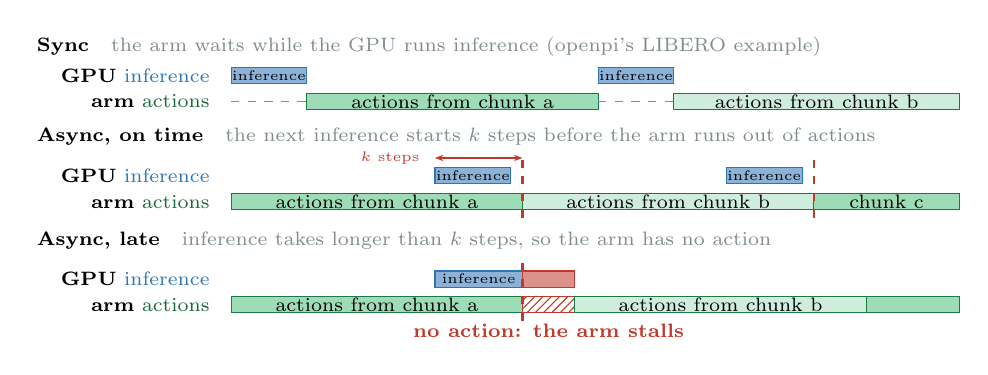
\begin{tikzpicture}[x=3.7mm, y=4.1mm, every node/.style={font=\scriptsize}]
  \tikzset{gpu/.style={fill=accent!55, draw=accent}, cha/.style={fill=green2!45, draw=green2!70!black}, chb/.style={fill=green2!22, draw=green2!70!black}}

  % ---- sync ----
  \node[anchor=west] at (-7,8.0) {\textbf{Sync}\quad\textcolor{gray2}{the arm waits while the GPU runs inference (openpi's LIBERO example)}};
  \node[anchor=east] at (-0.4,7.1) {\textbf{GPU}\ \textcolor{accent}{inference}};  \node[anchor=east] at (-0.4,6.3) {\textbf{arm}\ \textcolor{green2!60!black}{actions}};
  \draw[gpu] (0,6.85) rectangle (2.6,7.35);  \draw[gpu] (12.6,6.85) rectangle (15.2,7.35);
  \node[font=\tiny] at (1.3,7.1) {inference};  \node[font=\tiny] at (13.9,7.1) {inference};
  \draw[cha] (2.6,6.05) rectangle (12.6,6.55);  \node at (7.6,6.3) {actions from chunk a};
  \draw[chb] (15.2,6.05) rectangle (25,6.55);   \node at (20.1,6.3) {actions from chunk b};
  \draw[gray2, dashed] (0,6.3) -- (2.6,6.3);  \draw[gray2, dashed] (12.6,6.3) -- (15.2,6.3);

  % ---- async, on time ----
  \node[anchor=west] at (-7,5.2) {\textbf{Async, on time}\quad\textcolor{gray2}{the next inference starts $k$ steps before the arm runs out of actions}};
  \node[anchor=east] at (-0.4,4.0) {\textbf{GPU}\ \textcolor{accent}{inference}};  \node[anchor=east] at (-0.4,3.2) {\textbf{arm}\ \textcolor{green2!60!black}{actions}};
  \draw[gpu] (7,3.75) rectangle (9.6,4.25);  \draw[gpu] (17,3.75) rectangle (19.6,4.25);
  \node[font=\tiny] at (8.3,4.0) {inference};  \node[font=\tiny] at (18.3,4.0) {inference};
  \draw[cha] (0,2.95) rectangle (10,3.45);   \node at (5,3.2) {actions from chunk a};
  \draw[chb] (10,2.95) rectangle (20,3.45);  \node at (15,3.2) {actions from chunk b};
  \draw[cha] (20,2.95) rectangle (25,3.45);  \node at (22.5,3.2) {chunk c};
  \foreach \x in {10,20} { \draw[red2, dashed, line width=0.8pt] (\x,2.7) -- (\x,4.75); }
  \draw[{Stealth[length=3pt]}-{Stealth[length=3pt]}, red2, line width=0.6pt] (7,4.55) -- (10,4.55);
  \node[font=\tiny, text=red2, anchor=east] at (6.8,4.55) {$k$ steps};

  % ---- async, late ----
  \node[anchor=west] at (-7,2.0) {\textbf{Async, late}\quad\textcolor{gray2}{inference takes longer than $k$ steps, so the arm has no action}};
  \node[anchor=east] at (-0.4,0.8) {\textbf{GPU}\ \textcolor{accent}{inference}};  \node[anchor=east] at (-0.4,0.0) {\textbf{arm}\ \textcolor{green2!60!black}{actions}};
  \draw[gpu] (7,0.55) rectangle (10,1.05);  \node[font=\tiny] at (8.5,0.8) {inference};
  \draw[fill=red2!55, draw=red2] (10,0.55) rectangle (11.8,1.05);
  \draw[cha] (0,-0.25) rectangle (10,0.25);   \node at (5,0) {actions from chunk a};
  \draw[pattern=north east lines, pattern color=red2, draw=red2] (10,-0.25) rectangle (11.8,0.25);
  \draw[chb] (11.8,-0.25) rectangle (21.8,0.25);  \node at (16.8,0) {actions from chunk b};
  \draw[cha] (21.8,-0.25) rectangle (25,0.25);
  \draw[red2, dashed, line width=0.8pt] (10,-0.5) -- (10,1.5);
  \node[font=\scriptsize\bfseries, text=red2, anchor=north] at (10.9,-0.3) {no action: the arm stalls};
\end{tikzpicture}}
\end{center}

\vspace{0.1cm}
\begin{center}
\large Inference must finish before the arm runs out of actions.\\[0.2em]
If it doesn't, the arm stops.
\end{center}

\vspace{0.2cm}
\scriptsize\color{gray2}
LIBERO runs at 20 Hz, so starting 2, 3 or 5 steps early gives 100, 150 or 250 ms.

\end{frame}

% ==================================================================
\begin{frame}{What goes in, what comes out.}

\inrow

{\small\bfseries Out}\par\vspace{0.1cm}
\small
\begin{itemize}
  \setlength{\itemsep}{0.35em}
  \item End-to-end latency of every request, from \ts{1} to \ts{5}.
  \item The breakdown: travel, wait, run and travel back.
  \item Deadline miss rate, and p50 and p99 latency.
  \item Queue length for space, stall time for the robot.
  \item Alongside: GPU timeline, power, clocks and temperature.
\end{itemize}

\end{frame}

% ==================================================================
\begin{frame}{What we change, one at a time.}

\begin{center}
\small
\renewcommand{\arraystretch}{1.22}
\begin{tabular}{>{\raggedright\arraybackslash}p{0.2\linewidth}|>{\raggedright\arraybackslash}p{0.34\linewidth}|>{\raggedright\arraybackslash}p{0.34\linewidth}}
\toprule
& \textbf{Space} & \textbf{Robot} \\
\midrule
Other jobs & none, then other EO apps, then CPU and memory stress & none, then a perception model, then CPU and memory stress \\
Load & 1, 3 or 9 images every 1.5 s, one per satellite & fixed, one request per chunk \\
Budget & 1.5 s & 2, 3 or 5 steps (100, 150, 250 ms) \\
Precision & vLLM: 4-bit, then 8-bit & openpi: BF16, FP8, FP8 + NVFP4 \\
Batching & one at a time, then vLLM's batching & one at a time \\
Power mode & full power, then lower modes & same \\
\bottomrule
\end{tabular}
\end{center}

\vspace{0.3cm}
\small
Each run changes one row from the model-alone baseline.

\end{frame}

% ==================================================================
\begin{frame}{What we hold fixed.}

\vspace{-0.1cm}
\begin{center}
\footnotesize
\renewcommand{\arraystretch}{1.18}
\begin{tabular}{>{\raggedright\arraybackslash}p{0.2\linewidth}|>{\raggedright\arraybackslash}p{0.34\linewidth}|>{\raggedright\arraybackslash}p{0.34\linewidth}}
\toprule
& \textbf{Space} & \textbf{Robot} \\
\midrule
Image size & $896\times896$, pan and scan off & $224\times224$ \\
Output length & exactly 1 token, keep or drop & 10 actions, 10 denoising steps \\
Prompt & same text every time & same text, padded by openpi \\
Randomness & greedy, fixed seed & fixed noise seed \\
Inputs & \multicolumn{2}{>{\raggedright\arraybackslash}p{0.7\linewidth}}{synthetic, a new image every request so no cache can reuse work, same seed each run} \\
Sim machine & \multicolumn{2}{>{\raggedright\arraybackslash}p{0.7\linewidth}}{to be investigated} \\
Clocks & \multicolumn{2}{>{\raggedright\arraybackslash}p{0.7\linewidth}}{pinned with \texttt{nvpmodel} and \texttt{jetson\_clocks}, logged with \texttt{tegrastats}} \\
Warm-up & \multicolumn{2}{>{\raggedright\arraybackslash}p{0.7\linewidth}}{first requests thrown out, every run starts at the same temperature} \\
Software & \multicolumn{2}{>{\raggedright\arraybackslash}p{0.7\linewidth}}{one version of openpi and vLLM, one checkpoint each} \\
\bottomrule
\end{tabular}
\end{center}

\vspace{0.2cm}
\small
Then any spread we see comes from the system, not the inputs.

\end{frame}

% ==================================================================
\begin{frame}{Checking our setup.}

\vspace{0.6cm}
\begin{columns}[T,onlytextwidth]
\column{0.31\textwidth}
\begin{block}{Noise floor}
  \small
  Run a fake model that always takes exactly 50~ms. Any spread we see is our setup's own noise.
\end{block}
\column{0.31\textwidth}
\begin{block}{Inputs don't matter}
  \small
  Run once with real images. If the times match the synthetic run, synthetic is fine.
\end{block}
\column{0.31\textwidth}
\begin{block}{Add up}
  \small
  Travel, wait, run and travel back should add up to \ts{5} minus \ts{1}.
\end{block}
\end{columns}

\end{frame}

% ==================================================================
\appendix

% ==================================================================
% Possible directions: four candidate slides (ideal vs real). Keep the ones you want.
\begin{frame}[plain]
  \vfill
  \begin{center}
    {\Large\bfseries Possible directions.}\\[0.8em]
    \small KV-cache management and scaling speculative decoding.
  \end{center}
  \vfill
\end{frame}

% ------------------------------------------------------------------
% A. More GPUs hit a floor.
\begin{frame}{More GPUs do not buy one user much speed.}

\vspace{0.1cm}
\begin{center}
\resizebox{0.86\linewidth}{!}{%
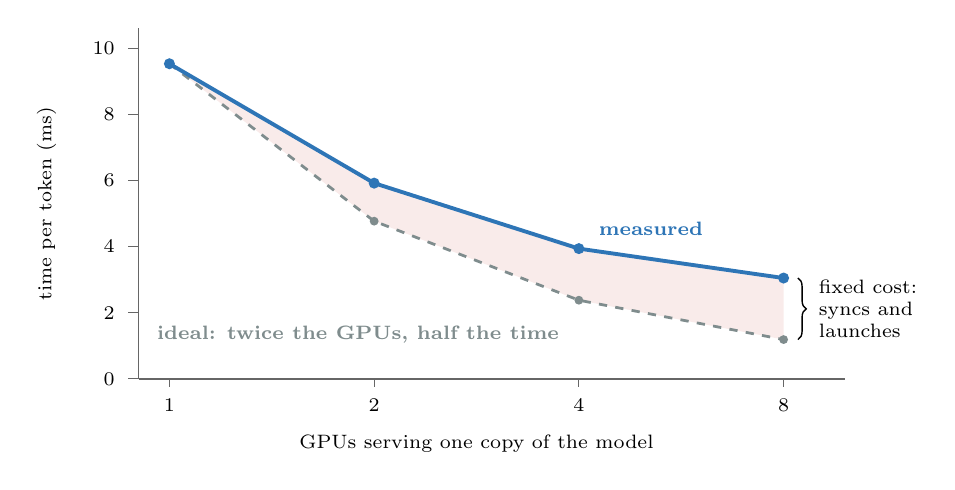
\begin{tikzpicture}[x=2.6cm, y=0.42cm, every node/.style={font=\scriptsize}]
  % axes
  \draw[black!60, line width=0.5pt] (-0.15,0) -- (3.3,0);
  \draw[black!60, line width=0.5pt] (-0.15,0) -- (-0.15,10.6);
  \foreach \x/\l in {0/1,1/2,2/4,3/8} { \draw[black!60] (\x,0) -- (\x,-0.25); \node[anchor=north] at (\x,-0.3) {\l}; }
  \node[anchor=north] at (1.5,-1.4) {GPUs serving one copy of the model};
  \foreach \y in {0,2,4,6,8,10} { \draw[black!60] (-0.15,\y) -- (-0.2,\y); \node[anchor=east] at (-0.22,\y) {\y}; }
  \node[rotate=90] at (-0.6,5.3) {time per token (ms)};
  % the gap between real and ideal
  \fill[red2!10] (0,9.53) -- (1,5.92) -- (2,3.94) -- (3,3.05) -- (3,1.19) -- (2,2.38) -- (1,4.77) -- cycle;
  % ideal: twice the GPUs, half the time
  \draw[gray2, dashed, line width=1pt] (0,9.53) -- (1,4.77) -- (2,2.38) -- (3,1.19);
  \foreach \x/\y in {1/4.77,2/2.38,3/1.19} \fill[gray2] (\x,\y) circle (1.6pt);
  % measured
  \draw[accent, line width=1.4pt] (0,9.53) -- (1,5.92) -- (2,3.94) -- (3,3.05);
  \foreach \x/\y in {0/9.53,1/5.92,2/3.94,3/3.05} \fill[accent] (\x,\y) circle (2pt);
  \node[accent, font=\scriptsize\bfseries, anchor=south west] at (2.05,4.05) {measured};
  \node[gray2, font=\scriptsize\bfseries, anchor=north east] at (1.95,1.9) {ideal: twice the GPUs, half the time};
  \draw[decorate, decoration={brace, amplitude=3pt}, line width=0.5pt] (3.07,3.05) -- (3.07,1.19)
    node[midway, right=4pt, align=left] {fixed cost:\\syncs and\\launches};
\end{tikzpicture}}
\end{center}

\vspace{0.1cm}
\small
Eight GPUs give 3.1 times the speed, not 8. Every token pays a fixed cost that more GPUs never shrink.\\[0.4em]
Speculation cuts the number of steps instead of the time per step.

\vfill
{\scriptsize\color{gray2}Llama-2-7B on A100, one request at a time. Source: gpt-fast README (PyTorch).}

\end{frame}

% ------------------------------------------------------------------
% B. Speculation's gain shrinks with batch.
\begin{frame}{Speculation's gain shrinks as the batch grows.}

\vspace{0.1cm}
\begin{center}
\resizebox{0.9\linewidth}{!}{%
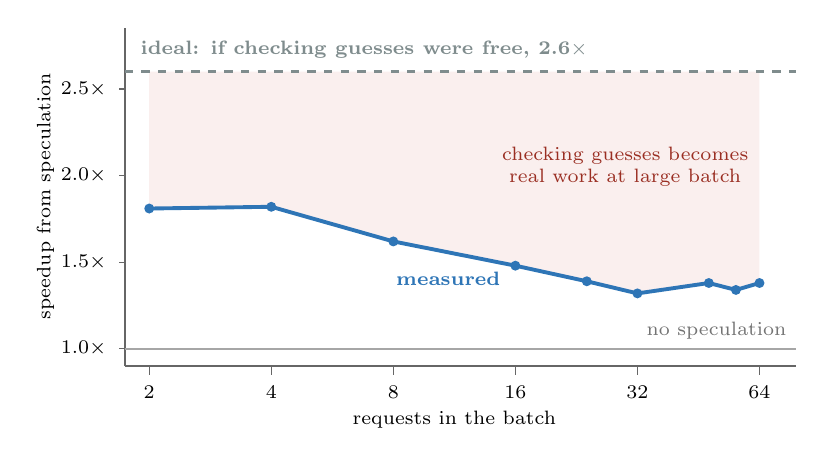
\begin{tikzpicture}[x=1.55cm, y=2.2cm, every node/.style={font=\scriptsize}]
  % axes (y starts at 0.9x)
  \draw[black!60, line width=0.5pt] (-0.2,0.9) -- (5.3,0.9);
  \draw[black!60, line width=0.5pt] (-0.2,0.9) -- (-0.2,2.85);
  \foreach \x/\l in {0/2,1/4,2/8,3/16,4/32,5/64} { \draw[black!60] (\x,0.9) -- (\x,0.85); \node[anchor=north] at (\x,0.84) {\l}; }
  \node[anchor=north] at (2.5,0.7) {requests in the batch};
  \foreach \y/\l in {1.0/1.0,1.5/1.5,2.0/2.0,2.5/2.5} { \draw[black!60] (-0.2,\y) -- (-0.25,\y); \node[anchor=east] at (-0.27,\y) {\l$\times$}; }
  \node[rotate=90] at (-0.85,1.88) {speedup from speculation};
  % no speculation
  \draw[black!35, line width=0.6pt] (-0.2,1.0) -- (5.3,1.0);
  \node[black!55, anchor=south east] at (5.3,1.0) {no speculation};
  % gap
  \fill[red2!8] (0,1.81) -- (1,1.82) -- (2,1.62) -- (3,1.48) -- (3.585,1.39) -- (4,1.32) -- (4.585,1.38) -- (4.807,1.34) -- (5,1.38) -- (5,2.6) -- (0,2.6) -- cycle;
  % ideal
  \draw[gray2, dashed, line width=1pt] (-0.2,2.6) -- (5.3,2.6);
  \node[gray2, font=\scriptsize\bfseries, anchor=south west] at (-0.15,2.62) {ideal: if checking guesses were free, 2.6$\times$};
  % measured
  \draw[accent, line width=1.4pt] (0,1.81) -- (1,1.82) -- (2,1.62) -- (3,1.48) -- (3.585,1.39) -- (4,1.32) -- (4.585,1.38) -- (4.807,1.34) -- (5,1.38);
  \foreach \x/\y in {0/1.81,1/1.82,2/1.62,3/1.48,3.585/1.39,4/1.32,4.585/1.38,4.807/1.34,5/1.38} \fill[accent] (\x,\y) circle (1.8pt);
  \node[accent, font=\scriptsize\bfseries, anchor=north] at (2.45,1.5) {measured};
  \node[align=center, text=red2!80!black] at (3.9,2.05) {checking guesses becomes\\real work at large batch};
\end{tikzpicture}}
\end{center}

\vspace{0.1cm}
\small
Checking guesses is nearly free only while the GPU has spare time.\\[0.4em]
As the batch grows, that spare time runs out and the gain falls.

\vfill
{\scriptsize\color{gray2}EAGLE-3 (arXiv 2503.01840) Table 3: Llama-3.1-8B, H100, SGLang, 3 guessed tokens. Ideal uses the acceptance measured in vLLM PR 35158.}

\end{frame}

% ------------------------------------------------------------------
% C. The same curve, with KV-memory limits.
\begin{frame}{KV memory decides whether speculation scales.}

\begin{center}
\resizebox{0.8\linewidth}{!}{%
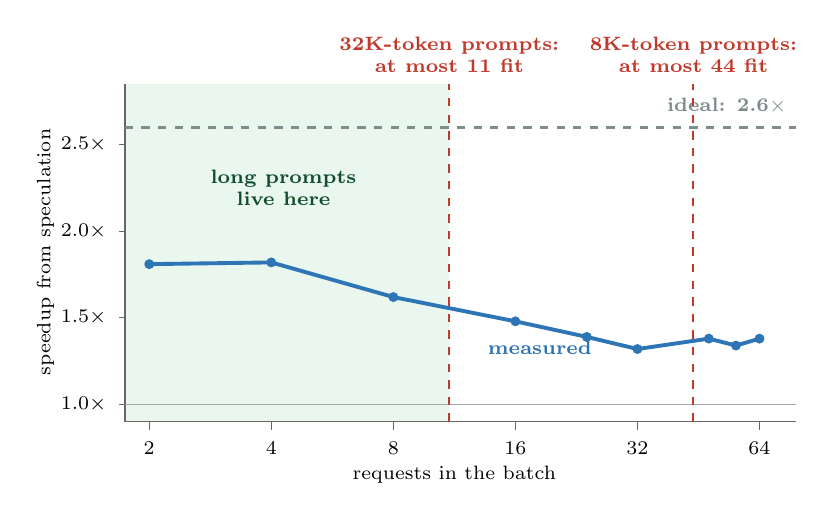
\begin{tikzpicture}[x=1.55cm, y=2.2cm, every node/.style={font=\scriptsize}]
  % where long prompts live
  \fill[green2!10] (-0.2,0.9) rectangle (2.459,2.85);
  % axes
  \draw[black!60, line width=0.5pt] (-0.2,0.9) -- (5.3,0.9);
  \draw[black!60, line width=0.5pt] (-0.2,0.9) -- (-0.2,2.85);
  \foreach \x/\l in {0/2,1/4,2/8,3/16,4/32,5/64} { \draw[black!60] (\x,0.9) -- (\x,0.85); \node[anchor=north] at (\x,0.84) {\l}; }
  \node[anchor=north] at (2.5,0.7) {requests in the batch};
  \foreach \y/\l in {1.0/1.0,1.5/1.5,2.0/2.0,2.5/2.5} { \draw[black!60] (-0.2,\y) -- (-0.25,\y); \node[anchor=east] at (-0.27,\y) {\l$\times$}; }
  \node[rotate=90] at (-0.85,1.88) {speedup from speculation};
  \draw[black!35, line width=0.6pt] (-0.2,1.0) -- (5.3,1.0);
  % ideal
  \draw[gray2, dashed, line width=1pt] (-0.2,2.6) -- (5.3,2.6);
  \node[gray2, font=\scriptsize\bfseries, anchor=south east] at (5.3,2.62) {ideal: 2.6$\times$};
  % memory limits (estimated, 80 GB H100)
  \draw[red2, dashed, line width=0.7pt] (2.459,0.9) -- (2.459,2.85);
  \draw[red2, dashed, line width=0.7pt] (4.459,0.9) -- (4.459,2.85);
  \node[red2, font=\scriptsize\bfseries, anchor=south, align=center] at (2.459,2.86) {32K-token prompts:\\at most 11 fit};
  \node[red2, font=\scriptsize\bfseries, anchor=south, align=center] at (4.459,2.86) {8K-token prompts:\\at most 44 fit};
  \node[green2!45!black, font=\scriptsize\bfseries, align=center] at (1.1,2.25) {long prompts\\live here};
  % measured
  \draw[accent, line width=1.4pt] (0,1.81) -- (1,1.82) -- (2,1.62) -- (3,1.48) -- (3.585,1.39) -- (4,1.32) -- (4.585,1.38) -- (4.807,1.34) -- (5,1.38);
  \foreach \x/\y in {0/1.81,1/1.82,2/1.62,3/1.48,3.585/1.39,4/1.32,4.585/1.38,4.807/1.34,5/1.38} \fill[accent] (\x,\y) circle (1.8pt);
  \node[accent, font=\scriptsize\bfseries, anchor=north] at (3.2,1.42) {measured};
\end{tikzpicture}}
\end{center}

\vspace{0.1cm}
\small
Long prompts fill KV memory, so batches stay small, which is where speculation still pays.\\[0.4em]
Possible direction: manage KV memory to keep speculation in that region.

\vfill
{\scriptsize\color{gray2}Measured curve: EAGLE-3 Table 3 (Llama-3.1-8B, H100). Batch limits are our estimate for the same model on an 80 GB H100, at 132 KiB of KV per token.}

\end{frame}

% ------------------------------------------------------------------
% D. Reserved but empty KV memory under a prefill/decode split.
\begin{frame}{The decode GPU holds memory before the data arrives.}

\vspace{0.1cm}
\begin{center}
\resizebox{0.86\linewidth}{!}{%
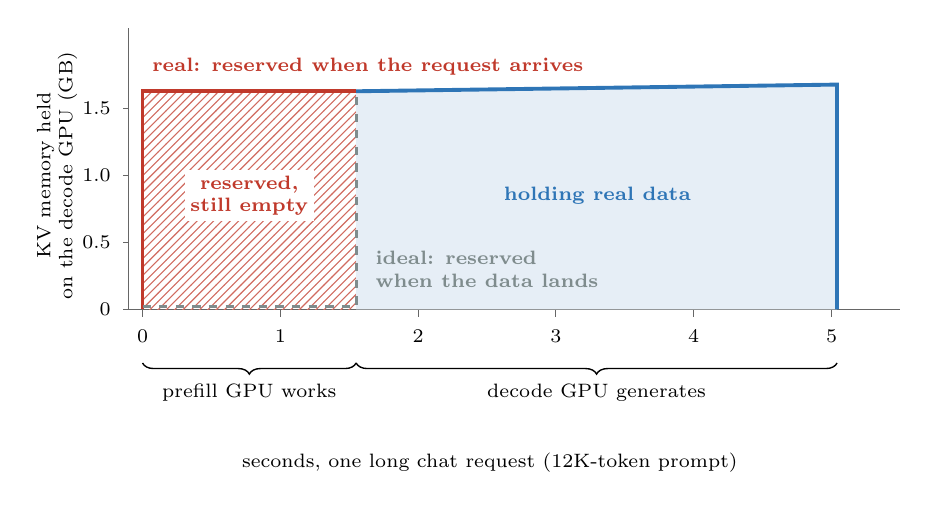
\begin{tikzpicture}[x=1.75cm, y=1.7cm, every node/.style={font=\scriptsize}]
  % axes
  \draw[black!60, line width=0.5pt] (-0.1,0) -- (5.5,0);
  \draw[black!60, line width=0.5pt] (-0.1,0) -- (-0.1,2.1);
  \foreach \x in {0,1,2,3,4,5} { \draw[black!60] (\x,0) -- (\x,-0.06); \node[anchor=north] at (\x,-0.08) {\x}; }
  \node[anchor=north] at (2.52,-1.0) {seconds, one long chat request (12K-token prompt)};
  \foreach \y in {0,0.5,1.0,1.5} { \draw[black!60] (-0.1,\y) -- (-0.14,\y); \node[anchor=east] at (-0.16,\y) {\y}; }
  \node[rotate=90, align=center] at (-0.62,1.0) {KV memory held\\on the decode GPU (GB)};
  % reserved but empty
  \fill[pattern=north east lines, pattern color=red2!75] (0,0) rectangle (1.55,1.63);
  \fill[accent!12] (1.55,0) -- (1.55,1.63) -- (5.04,1.68) -- (5.04,0) -- cycle;
  \node[fill=white, inner sep=2pt, text=red2, font=\scriptsize\bfseries, align=center] at (0.775,0.85) {reserved,\\still empty};
  \node[text=accent, font=\scriptsize\bfseries] at (3.3,0.85) {holding real data};
  % real and ideal lines
  \draw[red2, line width=1.4pt] (0,0) -- (0,1.63) -- (1.55,1.63);
  \draw[accent, line width=1.4pt] (1.55,1.63) -- (5.04,1.68) -- (5.04,0);
  \draw[gray2, dashed, line width=1pt] (0,0.02) -- (1.55,0.02) -- (1.55,1.63);
  \node[red2, anchor=south west, font=\scriptsize\bfseries] at (0,1.68) {real: reserved when the request arrives};
  \node[gray2, anchor=west, font=\scriptsize\bfseries, align=left] at (1.62,0.3) {ideal: reserved\\when the data lands};
  % phases
  \draw[decorate, decoration={brace, amplitude=4pt, mirror}, line width=0.5pt] (0,-0.4) -- (1.55,-0.4) node[midway, below=4pt] {prefill GPU works};
  \draw[decorate, decoration={brace, amplitude=4pt, mirror}, line width=0.5pt] (1.55,-0.4) -- (5.04,-0.4) node[midway, below=4pt] {decode GPU generates};
\end{tikzpicture}}
\end{center}

\small
With prefill and decode on separate GPUs, the decode GPU sets memory aside before the data arrives.\\[0.4em]
For long chat prompts that is about 44\% more memory held per request, memory that could hold more requests or more guessed tokens.

\vfill
{\scriptsize\color{gray2}Estimate from our cost model: Llama-3.1-8B on A100. SGLang 0.5.21 always reserves early; vLLM's default (pull) connector reserves late.}

\end{frame}

% ==================================================================
\begin{frame}{Assumptions.}

\vspace{0.2cm}
\small
\begin{enumerate}
  \setlength{\itemsep}{0.6em}
  \item openpi serves $\pi_{0.5}$ and vLLM serves Gemma 3.
  \item Synthetic inputs are enough, since image sizes and output lengths are fixed.
  \item Late space images wait in the queue rather than being dropped.
  \item We only test transformers: Gemma 3 4B and $\pi_{0.5}$.
  \item The robot loop runs at LIBERO's 20 Hz.
\end{enumerate}

\vspace{0.5cm}
Still open: where the sim runs, and whether Gemma 3 image input works in vLLM on the Thor.

\end{frame}

% ==================================================================

\begin{frame}[shrink=10]{Sources}
\scriptsize
\begin{itemize}
  \setlength{\itemsep}{0.45em}
  \item NVIDIA Jetson AI Lab, \emph{OpenPi $\pi_{0.5}$ on Jetson Thor}, \url{https://www.jetson-ai-lab.com/tutorials/openpi_on_thor/}. JetPack 7.2, MAXN, \texttt{pi05\_libero}: BF16 132.00 $\pm$ 0.89 ms, FP8 + NVFP4 48.84 $\pm$ 0.16 ms.
  \item openpi, \url{https://github.com/Physical-Intelligence/openpi}. LIBERO client: \texttt{examples/libero/main.py}. \texttt{pi05\_libero}: \texttt{src/openpi/training/config.py}. Prompt padding: \texttt{src/openpi/models/tokenizer.py}.
  \item LIBERO, \url{https://github.com/Lifelong-Robot-Learning/LIBERO}. 20 Hz control: \texttt{libero/libero/envs/bddl\_base\_domain.py}.
  \item VLASH code, \url{https://github.com/mit-han-lab/vlash}. Starting inference $k$ steps early: \texttt{vlash/run.py}. J.~Tang et al., \emph{VLASH}, arXiv 2512.01031.
  \item N.~Bleier et al., \emph{Space Microdatacenters}, MICRO 2023, \url{https://passat.crhc.illinois.edu/micro23.pdf}. Frame period: Sec.~5. Satellites per node: Sec.~8, Table~8.
  \item vLLM metrics, \url{https://docs.vllm.ai/en/latest/design/metrics.html}. NAVI-Orbital, arXiv 2606.18271, Sec.~VI-B.
\end{itemize}
\end{frame}

\end{document}
